\chapter{EEG/MEG preprocessing --- Reference
  \label{Chap:eeg:preprocessing}} 

In this chapter we will describe the function and syntax of all 
SPM/MEEG preprocessing and display functions. This will be the most
detailed description of the functions in this
manual. Our goal is to provide a comprehensive description of how the
software can be used to preprocess M/EEG data up to the point where
one would use one the source reconstruction techniques or statistical
analysis of M/EEG channel data. 

These functions can be called either from SPM's graphical user
interface (GUI), from the matlab command line, or via the batch input
system. We recommend beginners to use the GUI first, because this will
prompt SPM to ask all relevant information which are needed to process
the data. The batch input system is meant to cover repetitive analyses
of data once the user knows what should be done, in which order. The
command line facilities are very useful for writing scripts, or using
SPM's history-to-script functionality to generate scripts
automatically. The command line use of SPM for M/EEG will require some
matlab knowledge.

For the command line, we follow the concept of providing only one
input argument to each function. This input argument is usually a 
structure (struct) that contains all input arguments as fields. This
approach has the advantage that the input does not need to follow a
specific input argument order. If an obligatory input argument is
missing, the function will invoke the GUI and ask the user for the
missing argument. When using the GUI, a function is called without any
input argument, i.e. SPM will ask for all input arguments. If using
the command line (e.g., with a script), you can specify all arguments
in advance and effectively use SPM/MEEG functions in batch mode. We
provide some sample batch script (\textit{histexample.m}) in the
\textit{man/example\_scripts/} folder of the SPM8-distribution.
\\
\\
In the following we will go through the conversion of the data, specifics of the M/EEG format 
in SPM8, how to properly enter additional information about the channels, how to call 
fieldtrip-functions from SPM, a complete reference of all methods and functions, 
how to use the display, and finally how to script and batch the preprocessing.

\section{Conversion of data}
The first step of any analysis is the conversion of data from its
native machine-dependent format to a matlab-based, common SPM
format. This format stores the data in a *.dat file and all other
information in a *.mat file. The *.mat file contains the data
structure D and the *.dat is the M/EEG data. The conversion facility
of SPM is based on the "fileio" toolbox
(http://www2.ru.nl/fcdonders/fieldtrip/doku.php?id=fieldtrip:development:fileio),
which is shared between SPM8, Fieldtrip and EEGLAB toolboxes and
jointly developed by the users of these toolboxes. At the moment most
common EEG and MEG data formats are supported. For some cases, it
might be necessary to install additional Matlab toolboxes. In this
case an error message will be displayed with a link where the
appropriate toolbox can be downloaded. If your data format is not recognized
by fileio, it will still try to read the file using the Biosig toolbox 
(http://biosig.sourceforge.net/), if available. This can work for some
EEG systems, particularly clinical ones. One of the consequences of using Biosig as 'fallback'
is that you may see error messages from Biosig or mentioning Biosig if your data 
format is not presently supported. In such a case you can extend the fileio toolbox 
and contribute your code to us. See fileio page for details.

In the following we will describe the GUI-version for conversion.
One could also convert data using the batch or a
script. After clicking on the Convert button of the M/EEG GUI you will
be asked to select the file to be converted. As a rule of thumb, if the
dataset consists of several files, the file containing the data (which
is usually the largest) should be selected. SPM can usually
automatically recognize the data format and apply the appropriate
conversion routine. However, in some cases there is not enough
information in the data file for SPM to recognize the format. This
will typically be the case for files with non-specific extensions
(*.dat, *.bin, *.eeg etc.). In these cases the header-, and not the
data-, file should be chosen for conversion and if it is recognized,
SPM will locate the data file automatically. Note that SPM8 can also
convert data in SPM5 format, where the the *.mat file should be
selected.

After the file is chosen, you will be asked (Define settings?) to
choose whether to define some settings for the conversion or 'just
read'.  The latter option was introduced to enable a simple and
convenient conversion of the data with no questions asked. The
resulting SPM M/EEG data file can then be explored with SPM's reviewing tool to
determine the appropriate conversion parameters for the future. If
the 'just read' option is chosen, SPM will try to convert the whole
dataset preserving as much data as possible. The other option - 'yes'
lets you control all features of the conversion to convert only
the data that will be used in subsequent processing.

If this option is chosen, the next question will be whether to read
the data as 'continuous' or as 'trials'. Note that some datasets do
not contain continuous data to begin with. These datasets can only be
converted with the 'trials' option.  

If the 'continuous' option is chosen you will be asked (Read
everything?) whether to convert the whole file (yes) or a subset of it
(no). If the answer is 'no' you will be asked to specify the time
window in seconds. Note that if a data file contains several
concatenated long segments (e.g., if the recording was paused
and then resumed) only one of these segments at a time can be
converted as continuous.  Therefore you should specify a time window
which does not cross the boundaries between segments.  

If the 'trial' option is selected, the next question will be where to
retrieve the information about trials. There are three options. If
'data' is chosen, SPM will attempt to look for information about
trials in the dataset. This option is suitable for datasets that are already epoched
or datasets which contain some information about trials. If 'define'
is selected, trials can be defined based on information about events
which appears in the file. The routine used for this option is
identical to the one used in epoching (see below) and the resulting
SPM file will be already epoched. The advantage of defining trials at
conversion is that only the necessary subset of the raw data is
converted. This is useful when the trials of interest are only a small
subset of the whole recording. After the trial definition is
completed, the results can be saved into a file. This file can be
later used instead of repeating the trial definition again. This is
done by selecting the third trial definition option - 'file'. 

The next question will be about which channels should be
converted. Five options are available. 'all' - convert 
all the available channels. 'meg', 'eeg' - automatically detect and
choose MEG and EEG channels respectively. These options may
not work correctly for some MEG and EEG systems because many
data formats do not provide information about what data were acquired
by a specific channel. However, the most common cases are supported.
'gui' - choose the channels to convert using a graphical interface. 
The overall selection of channels can be saved in a file and this
file can later be used by choosing the 'file' option.

The final question is by which name the new SPM EEG files should be
written to disk. By default SPM will add the prefix 'spm8\_' to the
name of the raw data file if the data is read as continuous and
'espm8\_' if the data is read by trials.  

SPM will now convert the data. This may take some time depending on
file size and a red bar will inform you about the progress.


\section{Converting arbitrary data}
It might be the case that your data is not in any standard format
but is only available as an ASCII or Excel file or as a variable
in Matlab workspace. Then you have two options depending on whether
you would be willing to use a Matlab script or want to only use GUI.
If you want to only use GUI, we suggest that you assemble your dataset
in EEGLAB (http://sccn.ucsd.edu/eeglab/) and then then save it and convert
to SPM as any other format. The developers of EEGLAB have invested a lot of efforts
into making it possible to build a dataset from scratch without using the command line
or scripts and we see no reason for reproducing the same functionality in SPM. 

If you are willing to write a simple Matlab script, the most straightforward way 
to convert your data would be to create a quite simple Fieldtrip raw data struct 
and then use SPM's \textit{spm\_eeg\_ft2spm} function to convert this struct to SPM dataset.
Missing information can then be supplemented using meeg methods and SPM functions.

Fieldtrip raw struct must contain the following fields:

\begin{itemize}
\item .fsample - sampling rate (Hz)
\item .trial - cell array of matrices with identical dimensions channels x time
\item .time - cell array of time vectors (in sec), the same length as the
        second dimension of the data. For SPM the time vectors must be identical.
\item .label - cell array of strings, list of channel labels. Same length as
        the first dimension of the data. 
\end{itemize}

An example script for converting LFP data can be found under
toolbox$\backslash$Neural\_Models$\backslash$ spm\_lfp\_txt2mat.m.

\section{The M/EEG SPM format}
The M/EEG format has changed from SPM5 to SPM8. There were many
reasons why we decided that it was time to radically change the
format. If you still have some data from your SPM5 analyses, you can
convert them to SPM8 (see above). 

Here some explanation why we changed the format. Previously, we placed
all header information into a struct, which was then stored in a
mat-file. When the data were read, the struct-file was put into
working memory, and the data, contained in the dat-file, was linked to 
the struct, using memory-mapping. We found that making a struct
available in working memory was highly problematic. This was because
users would manipulate the 
struct but sometimes introduced an error to the format (e.g., they
removed a few 
trials from the data but did not update all fields relating to the
total number of trials). This would generate hard-to-resolve errors
when trying to further process the now inconsistent data. To avoid
this in the future, we introduced two changes. The first is that
SPM8 now 
always does a consistency check when loading a file. This means, if,
for whatever reason, the data format was made inconsistent, SPM8 will
now report this as soon the user tries to load these data. SPM8 will
also report where the check flagged an inconsistency. If there is enough
information available to fix the inconsistency, it will be done on the fly.
For instance, you will ususally see some messages about missing information when
converting a file to SPM8 format. These messages are normal and if no 
error is generated they do not indicate a problem. Second,
when reading the data, we now convert the header struct to an object
and only then make it available in working memory. Generally, this
Matlab object can only be manipulated using standardized functions
(called methods), which makes it very hard to introduce any
inconsistency into SPM M/EEG data in the first place. Also, using
methods simplifies internal book-keeping, which makes it much easier
to program functions operating on the M/EEG object. For example, while
the SPM5 format kept a variable which contained the number of total
trials, the SPM8 object does not have this variable but a method that
returns the number of trials by simply counting how many trials of
data there are. This makes it easy for a programmer to, for example,
remove trials. There is no more need to update a number of trials
variable. Also there is no need to check for the presence of particular fields
in the struct in every SPM function. All the methods are guaranteed to work on
a valid object. There are many more simplications along these lines due to
the object and methods. In summary, the change in format resulted in a
much more robust, and usable data format.

\section{Preparing the data after conversion}
SPM tries to do its best to extract information automatically
from the various data formats. In some case it can also supplements
the converted dataset with information not directly present in the raw data.
For instance, SPM can recognize commong EEG setups (extended 1020, Biosemi, EGI)
based on channel labels and assigns 'EEG' channel type and default electrode locations
for these cases. However, there are data types which are either not yet supported in this way
or do not contain sufficient information for SPM to make the automatic choices.
Also the channel labels do not always correctly describe the actual electrode
locations in an experiment. In these case some information needs 
to be supplied by the user. Reading and linking this additional information with the data is the
purpose of the 'prep' interface. This interface is accessed by
selecting 'Prepare' from the 'Other' drop-down menu in the GUI.  A menu
(easily overlooked) will appear at the top of SPM's interactive 
window. The same functionality can also be accessed by pressing 'Prepare SPM file' in
the SPM M/EEG reviewing tool.

In this menu, an SPM M/EEG file can be loaded and saved using the 'File'
submenu. 'Channel types' submenu allows reviewing and
changing the channel types. Use the 'Review' option to examine the
presently set channel types. During conversion, SPM tries to do its
best to 'guess' the correct channel types but this can sometimes go
wrong, in particular for EEG data. To set a particular channel group
to some channel type, select this type from the menu. A list of all
channels will appear. Select the subset whose type you would like to
set. Ctrl and Shift buttons can be used to refine the selection. Press
OK to apply your choice. It is especially important to correctly specify
which are the EEG channels. MEG types are assigned automatically by SPM
and cannot be modified in GUI.  

The 'Sensors' submenu can be used to supply information about the
sensor positions to the file. This information is needed to perform 3D
source reconstruction and DCM analysis for EEG and MEG data. 
Sensor positions for MEG are extracted from the raw data automatically and are already present. For EEG,
sensor positions are usually measured by a special device (such as
Polhemus) and are not part of the dataset. Even if you do not
measure electrode positions routinely in your lab, we recommend to
perform at least one initial measurement with the electrode cap you
use and use the result as your standard template. In order for SPM to provide a meaningful
interpretation of the results of source reconstruction, it should link the coordinate
system in which sensor positions are originally represented to the coordinate system of
a structural MRI image (MNI coordinates). In general to link between two coordinate
systems you will need a set of at least 3 points whose coordinates are known in both systems.
This is a kind of 'Rosetta stone'  that can be used to convert a position of any point from one system
to the other. These points are called 'fiducials' and the process of providing SPM with all the necessary
information to create the 'Rosetta stone' for your data is called 'coregistration'. 
 The most commonly used fiducials are the nose bridge and the two pre-auricular points.
The coordinates of these points for SPM's standard template
image are hard-wired in SPM code. So if your provide the coordinates of these specific
points with your sensor positions, it will be enough for SPM. If you do not have these
fiducials but have other anatomical landmarks (for instance 3 EEG electrodes whose positions can
be easily marked on a structural image) it will be possible to use them for coregistration as well, but that will
require additional input from you. In addition, or as a replacement of fiducials a headshape measurement may be used.
This measurement is done by an operator moving his
digitizer pen around on the subject's scalp and generates many more data 
points than just 3 fiducials. EEG sensor and fiducial positions can be added to an 
SPM file using 'Load EEG sensors' menu. There are 3 options:

\begin{itemize}
\item	'Assign default' - assigning default sensor positions. If 
  this is possible, it will be done automatically at conversion
  but this option can be used to revert to default sensor positions 
  after making some changes. 

\item 'From a *.mat file' - this option is for the kind of files that
  were used in SPM5 and can also be used for any kind of locations without
  trying to get them into one of the standard formats. SPM will as for two 
  files. The file sensors file should contain an $N \times 3$ matrix, 
  where $N$ is the same as the number of channels whose type is set to 'EEG'
  and the order of the rows matches the order of these channels in the SPM file. 
  The fiducials file  that should contain a $K \times 3$ matrix, where $K$ 
  (usually 3) is the number of fiducials.  You will be then be asked to provide
  labels for these fiducials. They should appear in the same order as the rows
  in the file.

\item	'Convert locations file' - this option uses a function from
  the internal fileio toolbox that supports several common formats for
  EEG channel position specification such as *.sfp and
  BESA's *.elp. It can also read Polhemus files from FIL and FCDC. In general
  Polhemus devices do not have a standard data format so if you are using Polhemus
  at a different site is is most likely that your Polhemus file will not be recognized
  by SPM directly. You will need to convert it to another format.
  An *.sfp file is the easiest to create (for instance in Excel).
  It is just an ASCII file containing a column of
  channel labels and 3 columns of cartesian coordinates.
  Check http://www2.ru.nl/fcdonders/fieldtrip/doku.php?id=fieldtrip:dataformat
  for a complete list of supported formats. The file you are importing can also
  contain positions of fiducial points or any other named points that do not
  necessarily correspond to channels. The important thing is that there are
  coordinates for each channel that was assigned 'EEG' type. 

\end{itemize}


The fiducials for MEG are automatically loaded from the dataset. However, in some
MEG setups the situation is more complicated. For instance, it might be convenient 
to attach the coils marking MEG fiducials to the top of the head, where there are no
clear anatomical landmarks. In this kind of cases there should be an additional file measured with Polhemus-like
device that contains the positions of MEG fiducials and something that can be linked to a structural
image (either anatomical landmarks or a headshape) in the same coordinate system. The way SPM
handles this situation is in two steps. First, this additonal file is converted into the same
coordinate system in which MEG sensors are represented and it replaces the original MEG fiducials.
At a later stage having MEG sensors and fiducials/headshape in the same coordinate system SPM
uses the fiducials/headshape for coregistration with standard MRI template or subject's own structural image. 
If you can mark the points where your MEG fiducial coils were located on a structural image, the step
described below is not necessary. It is also possible that the digitizer measurement is stored with the
raw data. Then SPM will read it automatically. Otherwise, the additional fiducials/headshape file can be loaded
using the 'Load MEG Fiducials/Headshape' menu. The supported formats are the same as for electrode locations.
It is also possible to create a fiducials/headshape Matlab struct and store it in a *.mat file. This file will
also be recognized by SPM. The struct should be called 'shape' and it should contain the following fields:
shape.pnt - a $K \times 3$ matrix (possibly empty) with headshape points i.e. some points that are on the surface of the head
and have no labels, shape.fid.pnt - $M \times 3$ matrix with fiducial points i.e. points that have labels,
shape.fid.label - $M \times 1$ cell array of strings with the labels of the points in shape.fid.pnt. As mentioned
before $M$ should be at least 3 for the coregistration to work. 

If you did not use default 3D positions, after loading the sensor
positions you can perform coregistration of your sensors with SPM's
template head model. This initial alignment is helpful to verify that
the sensor information you supplied were interpreted correctly and
should also be done if you would like to generate a 2D sensor template
based on your 3D sensor positions (see below). The 2D-coordinates will
be used for displaying the data in a topologically meaningful way. This
is done using the 'Coregister' option. For details of how this option works
see the 3D source reconstruction chapter \ref{Chap:eeg:imaging}. 

The '2D Projection' menu deals with the generation of representative
2D-coordinates for the sensors. Note that generating 2D-coordinates is
not obligatory. If the 2D-coordinates are not specified, the sensors will
be, when displaying, presented in a default square grid. Missing out
on topographically meaningful 2D-coordinates might be useful when
working on few channels. The 2D-coordinates are also used for
producing scalp-level SPMs in voxel space when converting M/EEG data
to images for later statistical analysis (see below). If you are 
planning to do 3D source reconstruction or 
DCM, 2D-coordinates are not necessarily required. Also, you can load
2D-coordinates from a file (several example files are available in
the \textit{EEGtemplates} SPM directory). For EEG, 2D-coordinates can also
be generated by projecting the 3D sensor positions to a plane. This is done
automatically when default 3D coordinates can be assigned and also for MEG.
In case of custom EEG sensor positions coregistration should be performed first (see
above). The resulting 2D-coordinates are displayed in SPM's graphics 
window. You can modify these projected 2D-coordinates
manually by adding, deleting and moving sensors. To select a sensor,
click on its label. The label will change its color to green. If
you then click at a different location, the sensor will be
moved to this position. Note that, at this stage, SPM does not
check whether there is any correspondence between the labels of the
coordinates and the labels of the channels stored in the SPM
file. When you are satisfied with the 2D-coordinates, select 'Apply'  
from the menu and the coordinates will be assigned to EEG or MEG
channels according to their labels. Note that 2D-coordinates cannot 
be assigned to channels of other types than M/EEG.  

Remember to save the file using File/Save after you finished modifying
it using the prep interface. Your changes will not be saved
automatically. In case of envoking prep from the reviewing tool you should
press the 'OK' button that will appear at the buttom left of the interactive window and
then save the file with the 'Save' button of the reviewing tool. 

In the rare case that you neither have measured sensor locations,
or fiducials, and the supplied standard templates do not work for you,
you can also supply a so-called channel template file, which contains
all information necessary. However, remember, that if you do not
supply any 2D-coordinates, you can still use all SPM functions,
however, SPM will use 2D-coordinates laid out in a topographically not 
meaningful rectangular pattern.

A channel template file contains four variables:\\

\begin{tabular}{llcp{9cm}}
{\bf Nchannels} & &  - & The number of channels\\
{\bf Cnames}&  & - & A cell vector of channel names. Each cell can
contain either a string or a cell vector of strings. The latter allows
to have multiple versions of a given channel name. Case can be
ignored, i.e.~it doesn't matter whether channel names are in small or
capital letters.\\
{\bf Cpos} & & - & A $2 \times Nchannels$-matrix of channel
coordinates on a 2D plane. In $x$- and $y$-direction the minimum
coordinate must be $\leq 0.05$ and the maximum coordinate
must be $\geq 0.95$. \\ 
{\bf Rxy} & & - & A factor that determines the width of the display
plots to their height when displaying the data. Standard is 1.5. \\
\end{tabular}

Note that the channel template files and 3D coordinate files with labels
(such as *.sfp) can contain many more channel
labels than your data file. SPM searches, for each channel in the
data, through the labels in the channel template file. If the labels
match, the coordinate is used. 

\subsection{History}
This menu allows you to review all the pre-processing steps that have been applied
to a particular data file by functions that support the history functionality (see below).
This is useful when you are not sure how a particular file was processed. It is also possible
to export the processing steps or a subset of them to a Matlab script and use them as a template
for a repeating the same analysis or doing a different one. Note that if you only export a subset
of steps the resulting script is not guaranteed to work or produce the same result.

\section{Integration of SPM and Fieldtrip}
The SPM8 distribution includes the latest version of 'Fieldtrip' toolbox
(http://www2.ru.nl/fcdonders/fieldtrip/). FieldTrip is a Matlab
toolbox for MEG and EEG analysis that is being developed at the
F.C. Donders Centre (FCDC) together with collaborating
institutes. Fieldtrip functions can be used for many kinds of analysis
which are not supported in SPM proper. However, Fieldtrip
does not have extensive graphical user interface and its functionality
should be accessed by writing scripts. Full reference documentation
for Fieldtrip including example scripts is available at the Fieldtrip
website (http://www.ru.nl/neuroimaging/fieldtrip/). The SPM
distribution also contains some documentation, contained as help
comments in Fieldtrip functions. These can be found in the directory 
external/fieldtrip/private. Note that in order to prevent function
name clashes SPM calls its Fieldtrip functions via 

intermediate or 'wrapper' functions whose name always starts with
'ft\_'. This has the advantage that even if there is a different Fieldtrip
version in Matlab path from the one used by SPM, SPM will only use its own
version and incompatibilities will be avoided. To adapt a standard
Fieldtrip script for use with SPM you must add the prefix 'ft\_' 
to all Fieldtrip function names in the script.

Fieldtrip data structures can be converted to SPM EEG files using
the \textit{spm\_eeg\_ft2spm} function.  SPM M/EEG data, once loaded
with the function \textit{spm\_eeg\_load} can be converted to Fieldtrip
format using the method 'ftraw' (with syntax D.ftraw or ftraw(D)).

\section{Reading of data}
\label{sec:load}
If you use the GUI only, there is no need to read this
section because the functions called by the GUI will read the data
automatically. However, if you plan to write scripts and access the
data and header information more directly, this section should contain
all the necessary information to do so. 

An SPM8 for M/EEG file can be read using the \textit{spm\_eeg\_load}
function. Without any arguments a file requester asks for the name of
the file. With a string argument $P$, \textit{spm\_eeg\_load(P)} will
attempt to read a file with the name $P$. The behavior in this case is
identical to 'Just read' option in the GUI. The SPM-format stores the
binary data in a *.dat file. All header information are stored in a
*.mat file. This *.mat file contains a single struct named {\textit D}
which contains several fields. When using \textit{spm\_eeg\_load}, the
struct is transformed into an object, and the data are linked into this
object. The linking is done via memory mapping using \textit{file\_array}
objects. Note that the data should always be read using the routine 
{\textit spm\_eeg\_load}. The memory mapped data can be
addressed like a matrix (see below) which is convenient for accessing
the data in a random access way. However, a word of caution: If you
write new values to this matrix, the matrix is not only changed
in the object (in memory), but also physically on the hard
disk.  

You can also load the header struct using a
simple \textit{load} but this just returns the header struct, without the
data linked in, and any spm-functions won't know what to do with this
struct.  In the following, we will describe the methods
that one can use on an M/EEG-object. Note that we will not describe
the internal format of the data here. This would be helpful only for
programmers who want to write new methods for meeg object, because when simply
analyzing M/EEG or even writing spm functions there should never be a need
to access the internal format. If you think that the existing methods do not
provide the functionality you need, please let us know. For interested power users,
there is documentation about the internal format within the meeg-class function 
\textit{meeg}. 

\subsection{Syntax}
\textit{D = spm\_eeg\_load(P)}
\\

\subsubsection{Input}
The input string {\textit P} is optional and contains the file name of the
*.mat file.

\subsubsection{Output}
The output struct {\textit D} contains all header information about the
data. The data are memory mapped and can be accessed directly using
something like \textit{d = D(:,:,1)}. This command would put the first
trial over all channels and time points into the variable $d$. The
first dimension of $D$ is channels, the second peri-stimulus time, and
the third is trials. If the data are time-frequency transformed, there
would be four dimensions, where the frequency dimension is squeezed in
at the second position (i.e., channels/frequencies/time/trials). If
you wanted to change the values of the data, you would write something
like \textit{D(1,2,3) = 1;}, which would change the value of the first
channel, second time-point, and third trial to 1.


\section{Methods for the M/EEG object}
M/EEG methods are functions that operate on an M/EEG object, loaded
with \textit{spm\_eeg\_load}. These methods should not be used, if you just
want to analyze your data using the GUI or simple scripts. However, if
you write your own scripts or high-level functions that need to read
or manipulate the object, you need the methods. In the following, we
will provide details about most of the methods, which appear to be
stable by the beta-release date. The code for all methods
can be found in the \textit{@meeg} SPM directory. Most methods provide
some minimalist help text. In the following, we will assume that the
object variable is called \textit{D}, i.e. previously load by using \textit{D
  = spm\_eeg\_load;}.

\subsection{Constructor meeg}
The \textit{meeg} method is a constructor. Called without any arguments it
will produce a consistent, but empty object. In SPM, the constructor
is called when a struct has been loaded into memory by
\textit{spm\_eeg\_load}, and is transformed into an
MEEG-object. Importantly, the constructor also checks the consistency
of the object. 

\subsection{display}
This method will return, in the matlab window, some information about
the object, e.g., \textit{display(D)}. 

\subsection{Number methods}
These are methods which return the number of something; they count the
number of channels, etc. For example, to find out how many channels an
MEEG object contains, you would use \textit{D.nchannels}, where $D$ is the
object. Number functions are \textit{nchannels, nfrequencies, nsamples,
  ntrials}.

\subsection{Reading and manipulation of information}
There are a large number of methods that can be used to either read or
write some information. The method name is the same but it depends on
the arguments whether something is read or stored. For example, when
you use the method \textit{badchannels}, you can either type
\textit{D.badchannels}, which returns the indices of all bad channels. You
could also change information about specific bad channels, e.g.,
\textit{D.badchannels([43:55], 1)} will flag channels 43 to 55 as
bad. You 
  could also use \textit{D.badchannels([43:55], ones(1,13)}, i.e. you
  can 
  either use a scalar to change all channels listed, or supply a
  0/1-flag for each channel. There are other functions which use the
  same logic. In the following we will list these functions and
  describe briefly what they do but won't go into much detail. We
  trust that you can work it out using the badchannels-example. 

\subsubsection{selectdata}
With this method the data can be indexed using channel labels, times and
condition labels instead of indices which you would usually need to find out
in your code. For instance D.selectdata('Cz', [0.1 0.12], 'Oddball') will return
the waveforms of channel Cz between 100 and 120 ms in peristimulus time for the
condition 'Oddball'

\subsubsection{chanlabels}
This method reads or writes the label of the channels (string).  Note that
the channel labels must be unique.

\subsubsection{chantype}
This method reads or writes the type of a channel (string). Currently,
the types recognized by SPM are: 'EEG', 'MEG', 'EMG', 'EOG', or
'Other', but in principle type can be any string.

\subsubsection{conditions}
This method  reads or writes the name of the condition of an epoch
(string). 

\subsubsection{events}
This method returns the events stored with each trial. Events are records
of things that happened during the experiment - stimuli, responses etc.
Before a file is epoched all the events are stored with the only trial and they 
can be used by the epoching function. For an epoched file SPM stores with each trial
the events that occured within that trials or possibly in some time window around it
(this is a parameter of the epoching function that can be specified). You can use this
information for your analysis (for instance to sort trials by reaction time). Events
are represented by a structure array with the following fields:

\begin{itemize}
\item .type - string (e.g. 'front panel trigger')
\item .value - number or string, can be empty (e.g. 'Trig 1').
\item .time - in seconds in terms of the original file
\item .duration - in seconds (optional)
\end{itemize}

Note that in order to find out the time of an event in peristimulus time
you will need additional information provided by 'trialonset' method.

\subsubsection{fname}
This method reads or writes the name of the mat-file, in which the
header information are stored. 

\subsubsection{fnamedat}
This method reads or writes the name of the dat-file, in which the
data are stored. 

\subsubsection{frequencies}
If the data has been transformed to time-frequency, this method reads
or writes the frequencies (Hz) of the data.

\subsubsection{fsample}
This method reads or writes the sampling rate of the data. In SPM, all
data must have the same sampling frequency.


\subsubsection{history}
This method can read or add to the history of a file. Usually, each
time a SPM function (e.g. like converting) does something to a data
set, the function name and arguments (possibly after collecting them
with the GUI) are stored in the history. Effectively, the history is a
documentation how exactly the data were processed. Of course, the
history function can also be used to replicate the processing, or
generate (modifiable) scripts for processing other data in the same
way.

\subsubsection{path}
This method reads or writes the path, under which the mat- and
dat-files are stored. 

\subsubsection{reject}
This method reads or writes the indices of rejected (bad) trials.

\subsubsection{timeonset}
This method reads and writes the time of the first sample in a trial
in peristimulus time (in seconds). In SPM all trials should have the
same time axis. Therefore there is only one timeonset in a file. For instance
if you have a pre-stimulus baseline of 100 ms and the stimulus comes at time zero,
timeonset will be -0.1. In general it is possible to define the time axis any way
you like and there is no requirement that the stimulus comes at 0 or that there
is baseline with negative times (which was the case in SPM5).

\subsubsection{trialonset}
This method should not be confused with the more commonly used 'timeonset' (above). 
It returns the times of the first sample of each trial in the original raw data
file time. This information is not always available to begin with. It may also be invalidated
during processing (for instance if you merge two epoched files). When this happens
the information is discarded. For SPM analysis trialonset is not usually necessary.
However it may be useful if you want to relate something in your analysis to the timing
of your experiment, for instance create a regressor for GLM analysis of single trials 
to account for fatigue. Trialonset is also necessary for interpretation of events in epoched
files.


\subsubsection{transformtype}
This method reads and writes the type of the data transform
(string). For example, when the data are transformed to a
time-frequency represention, the transformtype is set to 'TF'. For
time data, this is 'time'.

\subsubsection{type}
This method reads and writes the type of the data (string). Currently,
this string can be 'continuous', 'single', 'evoked', or 'grandmean'.

\subsubsection{units}
This method reads and writes the units of the measurements
(string). The units are channel-specific, i.e., each channel can have
its own units.


\subsection{Reading of information}
Some methods can only read information but not change them. These are:

\subsubsection{condlist}
This method returns a list of condition labels. Multiple entries of
labels have been removed.

\subsubsection{coor2D}
This method returns the 2D-coordinates used for displaying or writing
sensor data to voxel-based images.

\subsubsection{dtype}
This method returns the type under which the data are stored in the
file\_array object. 

\subsubsection{eogchannels}
This method returns which of the channels are EOG channels.

\subsubsection{indsample}
This method returns the index of the sample which is closest to a
specific time point (ms).

\subsubsection{meegchannels}
This method returns the indices of all channels that are either of the
MEG or EEG type. 

\subsubsection{modality}
This method returns the modality of channels (MEG, EEG, etc.).

\subsubsection{pickconditions}
This method returns the indices of trials of a certain condition. The
condition must be supplied by its label (string).

\subsubsection{repl}
This method returns the number of replications measured for a
condition. This method is usually only used on single trial data.

\subsubsection{time}
This method returns the time (ms) of the samples.

\subsubsection{sensors}
This method returns the sensor locations struct. There is an additional argument
for modality ('EEG' or 'MEG') as we are planning to support datasets with more
than one sensor type. The exact way sensors are represented depends on the modality
and you can find more information in Fieldtrip documentation as the sensors struct is
produced and used by code originally developed at FCDC. Note that in SPM sensors are not 
directly linked with channels, unlike for instance in EEGLAB. So there is no requirement
for the number of sensors and channels to match or even for any relation between them.
Of course loading sensors completely unrelated to your data will not be very useful and will
eventually lead to an error. This kind of representation is more powerful than a
simple correspondence and it will become even more useful with further development of SPM. 


\subsubsection{fiducials}
This method returns the fiducials. They are represented as 'shape' struct (see the
discussion of loading fiducials by the prep function) with an additional field for
units that is assigned automatically. 

\subsection{Manipulation of information}
There are two functions which only manipulate the objects. 

\subsubsection{ftraw}
This method converts an object to a fieldtrip struct. An additional
argument can be supplied to indicate whether the data is memory mapped
(1: default) or loaded into memory (0). Note that not all Fieldtrip functions
can properly handle memory mapped data. In order to avoid corrupting
the data, ftraw sets a read-only flag on it so in the worst case you might
encounter errors in Fieldtrip functions. Please report such errors on
SPM or Fieldtrip mailing list as we are interested in fixing them. ftraw(0) is 
safer in this respect but inefficient in its memory use. 

\subsubsection{save}
This method saves the object to the mat- and dat-files.

\subsection{struct-like interface}
In addition to pre-defined internal fields that should only be manipulated
using methods, meeg object also allows storing additional information in it
as long as the names of additional fields do not clash with the names of existing methods.
This functionality is used by some SPM functions. For instance, the results of 3D source
reconstructions are stored in D.inv field for which no methods are necessary
to access and modify it. You can use this functionality in your scripts (try commands like 
D.myfield = 'hellow world'; disp(D.myfield);). The methods rmfield and isfield work for these
extra-fields as they would if meeg object was a struct.

\section{SPM functions}
In this section we will describe the high-level SPM functions which
are used for preprocessing M/EEG data. These functions are fairly
standard and should allow a simple preprocessing of the data (e.g.,
epoching, filtering, averaging, etc.). Here, we will just describe
what each function roughly does and what the input arguments mean. More detailed information about the
syntax can be found in the help text of the code. For example, to get detailed help on epoching, type
\textit{spm\_eeg\_epochs}. The general syntax is the same for all
functions. If called from the command-line, and if no input arguments
are specified, the function will behave exactly as if you called the
function from the GUI by pressing a button or choosing it from the 'Other' menu. However, on the command line, or from a script,
you can supply input arguments, up to the point when all required input
arguments are specified, so that the function will run without any user
interaction. In this way, one can write a script that runs without
user interaction. See the folder \textit{man/example\_scripts} for an example. Input
arguments are provided in a struct $S$, whose 
fields contain the arguments. A typical call, e.g., from a script
would be: \textit{D = spm\_eeg\_epochs(S)}, where $S$ is the input
struct, and $D$ contains the return argument, the epoched MEEG object. Note that, with all SPM
functions, the object is also always written to hard disk. The filenames of the mat- and dat-files 
are generated by prepending a single letter to the old file
name. In the example of epoching this would be an 'e'. The idea is that
by calling a sequence of functions on a file, the list of first
letters of the file name shows (roughly) which preprocessing steps were
called to produce this file. Note that another way of calling SPM
functions and specifying all input parameters is to use the new batch
interface.

\subsection{Epoching the data: spm\_eeg\_epochs}
Epoching cuts out little chunks of continuous data and saves them as
'single trials'. In M/EEG research, this is a standard data selection
procedure to remove long gaps between each single trial. For each
stimulus onset, the epoched trial starts at some user-specified
pre-stimulus time and 
end at some post-stimulus time, e.g.~from -100 to 400 milliseconds in
peri-stimulus time. The epoched data will also be baseline-corrected,
i.e.~the mean of the pre-stimulus time is subtracted from the whole
trial. The resulting event codes are the same as saved in the *.mat
file. The prepended output letter is 'e'.

The epoching function can deal with two different ways of specifying trials 
you want to epoch. The first is to specify explicitly where each trial is located 
in the measured time-series. The second is to specify trials using the labeled events
stored in the file. For most users, the second way is the most convenient, but sometimes, when
the stored triggers in the file do not relate to what you want to epoch or there is no event
information available with in the raw data (e.g. when you have an external stimuli file),
you should use the first. 
\\
In the first input way, you specify a $N \times 2$ so-called \textit{trl}-matrix, where
each row contains the start and end of a trial. Optionally, there can be a third column 
containing the offset of the trigger with respect to the trial. An offset of 0 (default)
means that the first sample of the trial corresponds to the trigger. A positive offset indicates
that the first sample is later than the trigger, a negative offset indicates that the trial begins before the trigger
In SPM the offset should be the same for all trials. The need to specify a whole column is for interoperability
with Fieldtrip where trials can have different time axes. In addition you have to specify conditionlabels (a single string or a cell array
of strings), either one for each trial or one for all trials. You can also enter a 'padding' which will add time points before and after each 
trial to allow the user to later cut out this padding again. This is useful, e.g., for filtering epoched
data, where one would otherwise, without padding experience 'edge effects'. 

For the second input way, one should define the pre- and post-stimulus interval, and also specify
the events (triggers) around which the epochs will be 'cut'. SPM identifies events by their 'event type' and 
'event value'. These are strings or numbers 
which the software run by the EEG or MEG vendor uses when generating the measurement file. 
If you don't specify parameters for the epoching function, a GUI will pop up, and present
the found triggers with their type and value entries. These can sometimes look strange, 
but if you want to run a batch or script doing the epoching, you have to find out first what
the type and value of your event of interest are. Fortunately, these tend to be the same over scanning sessions, 
so that you can batch multi-subject epoching using the types and values found in one subject. 
You also have to come up with a 'condition label' for each trial type, which can be anything 
you choose. This is the label that SPM will use to indicate the trial type of a trial at later
processing stages. It is possible to use several types of triggers for defining trials with the
same label - in GUI just select several events using Shift or Ctrl key.

For both methods of input you also have to set a (0/1)-flag (no/yes) whether you 
want to review the information for all trials after selecting them, when you want
to make sure that all your trials are there. You should set the review-flag to 0,
if you write a non-interactive script. In GUI you can review a list of the epochs you defined
and exclude some of them by hand (e.g. only take the triggers from the first 5 min of recording).
You can also choose to save the trial definitions, for example, for re-use of another epoching of the same data.

\subsection{Filtering the data: spm\_eeg\_filter}
Continuous or epoched data can be filtered, over time, with a low-,
high-, stop- or bandpass-filter. SPM uses a Butterworth filter to do this. Note that
SPM uses the signal processing toolbox. This means that you have to
have this toolbox to filter data in SPM. Phase delays are minimised by
using matlab's {\textit filtfilt} function which filters the data
twice, forwards and backwards. The prepended output letter is 'f'.

When you use the function in GUI mode, it will automatically 
use the Butterworth-filter. You can then choose among four different 
ways of how you want to filter your data: Lowpass, highpass, bandpass,
and stopband. Depending on your choice, SPM will ask for the cutoff(s) in Hz.


\subsection{Artefact detection and rejection: spm\_eeg\_artefact}
Some trials not only contain neuronal signals of
interest, but also a large amount of signal from other sources like
eye movements or muscular activity. These signal components are
referred to as artefacts. In SPM, we use two simple automatic
artefact detection schemes. The first is thresholding the data and the
second is robust averaging. One can also choose to detect artefacts
manually by visualizing each trial using the display. Another option
is to use a more sophisticated artefact detection approach
(implemented by some other software) and supply that information to
SPM. 

Thresholding of the data is done in two passes. In the first pass, SPM
detects all instances, over trials and channels, where the
absolute value is higher than the threshold. If a channel has more
than a certain percentage of artefactual trials, it is defined as a
bad channel. In a second pass the thresholding is repeated, but
without taking into account any bad channels. A trial for which the
absolute data surpasses the treshold in some channel (excluding bad
channels) is then considered artefactual and flagged as a rejected
trial.

Note that the function only indicates which trials are artefactual or
clean and subsequent processing steps (e.g.~averaging) will take this 
information into account. However, no data is actually removed from
the *.dat file. The *.dat file is actually copied over without any
change. The prepended output letter is 'a'.

When you call the function, you are first asked whether you want
to read your own artefact list. This gives you the opportunity to 
tell SPM which of your trials are artefactual, and which are clean. 
The two lists of trial numbers don't need to be complete, i.e., you
can specify a few trials as artefactual or clean but SPM will still
check for artefacts in the remaining trials. 
The next question is whether you want to use robust averaging for your data.
This approach estimates weights, lying between 0 and 1, that indicate how much 
artefactual a trial is. Later on, when averaging to produce evoked responses, 
each trial is weighted by this number. For example, if the weight of 
a trial is close to zero, it doesn't have much influence in the average, 
and is effectively treated like an artefactual trial.If you choose
robust averaging, you first have to choose an offset for the weighting
function. This value, default value 3, defines the weighting function
used for averaging the data. The value 3 will roughly preserve 95\% of
data points drawn randomly from a Gaussian distribution. Next, one has
to specifiy the width of a smoothing kernel of the residuals. As
robust averaging treats each data point as independent it is necessary
to smooth the data after averaging. The value is specified in
milliseconds and its default is 20.

SPM will next ask whether you want to threshold your channels. If you
choose yes, 
you can then enter a list of channels, for which you want to check whether 
the absolute values of a trial surpass this threshold. Next, the threshold
itself can be either a vector of thresholds, i.e., one for each channel, 
or a single threshold, which SPM uses for all channels.

\subsection{Downsampling: spm\_eeg\_downsample}
The data can be downsampled to any sampling rate. This is useful if
the data was acquired at a higher sampling rate than one needs for 
making inferences about low-frequency components. For example,
resampling from 1000 Hz to 200 Hz would cut down the resulting file
size to 20\% of the original file size. Note that SPM's downsampling
routine uses the matlab function {\textit resample}, which is part of
the signal processing toolbox. The prepended output letter is 'd'.

Here, you choose the new sampling rate (Hz) which must be smaller than the old sampling rate.

\subsection{Rereferencing: spm\_eeg\_montage}
Sometimes it is necessary to re-reference the data to a new
reference. In SPM this is done by specifying a weight matrix, which 
pre-multiplies the data. This is a general approach which 
allows one to re-reference to the average over channels, to single
channels, or any linear combination of channels, e.g. the average over
a pair of channels. The prepended output letter is 'M'. Note that re-referencing
should mainly affect the analysis you do at the channel level and should have little
effect on 3D source reconstruction and DCM as long as it is not too noisy.

When you call the function, you will first be asked whether you want 
to use a GUI or information read from a file to specify the montage. 
If you choose GUI, you will see, on the left hand side, the montage-matrix,
where each row stands for a new channel. This means the labels in the left 
column describe the new labels. The old labels are on top, that means, each 
row contains weights for how the old channels must be weighted to produce a new 
channels in the montage. On the right hand side, you see a graphical represention 
of the current matrix. The default is the identity matrix, i.e., the montage will
not change anything. The concept is very general. For example, if you want to 
remove channels from the data, just delete the corresponding row from the montage matrix.
To re-reference to a particular channel the column for this channel should be -1 for
all rows, except the row corresponding to itself which should be 0, whereas the other channels 
should have 1 in the intersection of their column and row (the diagonal of the matrix) and 0 elsewhere.
For average reference the matrix should have (N-1)/N (where N is number of channels) at the diagonal and -1/N elsewhere.
In principle, any montage can be represented this way. If you are not sure about how to represent a montage you need,
ask an expert or write to SPM mailing list. The specification will only need to be done once for your setup and then you can
save the montage and use it routinely. When you changed the weights of the matrix, you can check the montage by pressing 
the button in the lower right below the figure.
\\
If you choose to specify the montage by 'file', you have to enter the filename of a mat-file, 
which contains a struct with 3 fields: 'labelnew' (labels of new channels), 'labelorg' (labels of original channels), 
and the montage-matrix 'tra' (tra as in transform).

Finally, you will be asked, whether you want to 'keep the other channels'. There may be channels that are
not involved in the montage. For instance, you apply montage defined for your EEG channels but there are also
EOG or trigger channels in the file. If you answer 'yes', they will just be copied to the new file unaffected.
If you answer 'no' they will not be included in the new file.


\subsection{Grand mean: spm\_eeg\_grandmean}
The grand mean is usually understood as the average of evoked
responses over subjects. The grand mean function in SPM is typically
used to do exactly this, but can also be used to average over multiple 
EEG files, e.g.~multiple sessions of a single subject. The averaged
file will be written to the same directory as the first selected
file. The prepended output letter is 'g'.

The function will ask you for the name of the output file. Note that in a
script, by default, when you don't specify an output filname, 
SPM will generate a new file with the filename of the first selected file, 
prepended with a 'g'.

\subsection{Merge: spm\_eeg\_merge}
Merging several MEEG files can be useful for concatenating multiple
sessions of a single subject. Another use is to merge files and then
use the display tool on the concatenated file to be able to display
data coming from different files in the same graph. This is the
preferred way in SPM to display data together that is split up into
several files. The merged file will be written into the same directory
as the first selected file. The prepended output letter is 'c'.

The function will first check whether there are at least two files,
and whether all data are consistent with each other, i.e., have the 
same number of channels, time points, and sampling rate. The function 
will also ask for a number of condition labels, one for each file and 
condition. This gives you the opportunity to rename labels. This might
be useful when you merge files which contain the same conditionlabels,
e.g. when you used several sessions for one subject but measured the 
same conditions in all files. In this case, it might be helpful to 
rename the conditions like 'condition A' to something like 'condition A, session 1', 
etc.



\subsection{Time-frequency decomposition: spm\_eeg\_tf}
\label{sec:tf}
The time-frequency decomposition uses a continuous
Morlet wavelet transform. The result is written to one or two result
files, one contains the instantaneous power and the other, optionally
written, the phase estimates. One can select the channels and
frequencies for which power and phase should be estimated. Optionally,
one can apply a baseline correction to the power estimates, i.e.~the
mean power of a pre-stimulus interval is subtracted from the power
estimates. For power, the prepended output letters are {\textit
  t1\_}, for phase {\textit t2\_}.

The function will first ask you, after selecting the M/EEG file, 
for a list of frequencies, which is a vector of numbers (Hz).
 For each of these frequencies, SPM will estimate the power and phase at each 
channel, time-point and trial. The next question is whether you want to remove 
the 'baseline' (i.e. the average power over some time-period in the pre-stimulus interval) 
from the time-frequency power estimates. If you choose yes, SPM will ask you for the time-period 
over which you want to form the baseline. Next, SPM will ask you for the so-called 
'Morelet Wavelet factor'. The default is 7. The greater this number, the less resolution you
 have over time, but the higher the resolution is in frequency. Then you can select the channels 
for which you want to compute the time-frequency decomposition. SPM will then ask you whether 
you also want to estimate the phase, in addition to power. The final question is whether you want
to 'collapse channels'. If yes, SPM will average the estimates (within power and phase) over all selected channels. 

\subsection{Averaging: spm\_eeg\_average}
Averaging of single trial data is the crucial step to obtain the
evoked response. By default, when averaging single trial data, single
trials are averaged within trial type. Power data of single trials
(see sec.~\ref{sec:tf}) can also be averaged by using the function
\textit{spm\_eeg\_average\_TF}. The preprended output letter is 'm'.


\subsection{Contrast of trials: spm\_eeg\_weight\_epochs}
As an extension to the averaging functionality, SPM can also be used
to compute linear combinations of single trials 
or evoked responses. For example, if you want to compute the
difference between two evoked responses, you supply a contrast vector
of $[-1; 1]$. Similarly, if you want to remove some trials from the
file, you can do this by using a contrast vector like $[1; 0]$ which
would write a new file with only the first evoked response. The
preprended output letter is 'm'. 

The function will first ask you to 'Enter contrasts'. 
This is a matrix where each contrast is given by a row of 
this matrix. For example, if you compute just one contrast,
you have to enter a vector of the same length as the number of 
trial types in the file. Note that SPM will zero-pad this vector
 (or matrix) if you specify less contrast weights than you have trials.
 The next question is whether you want to 'Weight by num replications'. 
This is important when you use this function on single trials, where, 
typically, you have a different number of trials for each trial type. 
If you then choose to average over multiple trials, this option allows 
you to choose whether you want to form an average that is weighted 
by the number of measurements within each trial type. As compared 
to an average, where you implicitly first form the averages within 
trial type, and then average with equal weighting.

\section{Displaying data with SPM EEG REVIEW}
Call from main SPM gui:    Display $\rightarrow$ M/EEG

SPM EEG REVIEW is meant to provide the user with basic visualization (data and source reconstruction) and reviewing (e.g. trial and sensor good/bad status) tools.

When called, SPM EEG REVIEW displays in the SPM graphics window information about the SPM data file which is displayed (only for matlab versions $>$ 7.1).

SPM EEG REVIEW uses tabs to easily access different fields in the SPM data file structure (see relevant SPM manual section for SPM EEG data format).
The main tabs system, at the top of the graphics windows, offers the following alternatives:

\begin{itemize}

\item{\textbf{EEG}}
displays EEG type data (if any). These are the data associated with 'EEG' sensors. This tab is described bellow, as well as the 'MEG' and 'OTHER' tabs (1- data visualization).
\item{\textbf{MEG}}
displays MEG type data (if any).

\item{\textbf{OTHER}}
displays any other type of data (e.g. HEOG, VEOG, etc�).

\item{\textbf{info}}
(active tab by default): displays basic information about the data file. This tab contains three further sub-tabs\footnote{User can also check sensor coregistration when clicking on 'sensor positions'.}: 'channels', 'trials' and 'inv' (the latter shows source reconstructions parameters, if any). Some of these infos can be changed by the user (e.g. sensor/trial\footnote{Sensor/trial status (good/bad) can also be changed under the EEG/MEG/OTHER tabs, when visualizing trials (sensor: right-click uicontextmenu ; trials: button 10).}  type, label and status, etc�) by editing the table. The changes become effective when clicking on 'update'. They are actually saved in the data file when clicking on 'SAVE'.

\item{\textbf{source}}
display source reconstructions (if any). See bellow (2- source reconstructions visualization).
\end{itemize}

In addition, the user can call the SPM EEG file preparation routine \footnote{This is part of the SPM EEG preprocessing tools. It mainly concerns the coregistration of the sensors onto the normalized SPM space. See relevant section in the SPM manual.} or save any modification in the data file suing the top-right buttons 'prepare SPM file' and 'SAVE'.


\subsection{Data visualization}
The graphics window of SPM EEG REVIEW offers two modes of data visualization: 'scalp' and 'standard' (default).
For continuous (non epoched) data, only 'standard' mode is enabled.
For time-frequency data, only 'scalp' mode is enabled.
For any other type of data, the user can switch to any of these modes using the standard/scalp radio button.
These two modes are described below:

\begin{itemize}
\item{\textbf{standard}}
channels are displayed vertically, within the same axes. A channel uicontextmenu can be accessed by right clicking on any time series (e.g. for changing the channel good/bad status). 
An additional axes (bottom right) provides the user with the temporal and horizontal scale of the displayed data).
The size of the plotted time window can be changed using the top left buttons 1 and 2. User can scroll through the data using the temporal slider, at the bottom of the graphics window. A global display scaling factor can be changed using the top buttons 3 and 4. Zooming within the data is done by clicking on button 5. Clicking on button 6 displays a 2D scalp projection of the data.

When displaying epoched data, the user can select the trial within the list of accessible trials (top right of the window). It is also possible to switch the status of trials (good/bad) by clicking on button 10.

When displaying continuous data, SPM EEG REVIEW allows the user to manage events and selections. After having clicked on button 7, the user is asked to add a new event in the data file, by specifying its temporal bounds (two mouse clicks within the display axes). Basic properties of any events can be accessed either in the 'info' table, or by right-clicking on the event marker (vertical line or patch superimposed on the displayed data). This gives access to the event uicontextmenu (e.g. for changing the event label).
Using buttons 8 and 9 allows the user to scroll through the data from marker to marker (backward and forward in time).

\item{\textbf{scalp}}
channels are displayed vertically, within the same axes. A channel uicontextmenu can be accessed by right clicking on any time series (e.g. for changing the channel good/bad status). 
An additional axes (bottom right) provides the user with the temporal and horizontal scale of the displayed data).
The size of the plotted time window can be changed using the top left buttons 1 and 2. User can scroll through the data using the temporal slider, at the bottom of the graphics window. A global display scaling factor can be changed using the top buttons 3 and 4. Zooming within the data is done by clicking on button 5. Clicking on button 6 displays a 2D scalp projection of the data.

When displaying epoched data, the user can select the trial within the list of accessible trials (top right of the window). It is also possible to switch the status of trials (good/bad) by clicking on button 10.

When displaying continuous data, SPM EEG REVIEW allows the user to manage events and selections. After having clicked on button 7, the user is asked to add a new event in the data file, by specifying its temporal bounds (two mouse clicks within the display axes). Basic properties of any events can be accessed either in the 'info' table, or by right-clicking on the event marker (vertical line or patch superimposed on the displayed data). This gives access to the event uicontextmenu (e.g. for changing the event label).
Using buttons 8 and 9 allows the user to scroll through the data from marker to marker (backward and forward in time).
\end{itemize}

\subsection{Source reconstructions visualization}
SPM EEG REVIEW makes use of sub tabs for any source reconstruction that has been stored in the data file\footnote{This concerns any distributed source reconstruction, i.e. also includes imaging DCM analyses, but not ECD reconstructions (so far).}. Since these reconstructions are associated with epoched data, the user can choose the trial he wants to display using the list of accessible events (top of the main tab).
Each sub tab has a label given by the corresponding source reconstruction comment which is asked to the user when source reconstructing the data (see relevant section in the SPM manual).
The bottom-left part of each sub tab displays basic infos about the source reconstruction (date, number of included dipoles, number of temporal modes, etc�).
The top part of the window displays a rendering of the reconstruction on the cortical surface that has been used. User can scroll through peri-stimulus time by using the temporal slider bellow the rendered surface. Other sliders allow the user to (i) change the transparence of the surface (left slider) and (ii) threshold the colormap (right sliders).
At the center is displayed a butterfly plot of the reconstructed intensity of cortical sources activity over peri-stimulus time.
If the data file contains more than one source reconstruction, the bottom-right part of the window displays a bar graph of the model evidences of each source reconstruction. This provides user with a -visual- Bayesian model comparison tool\footnote{Remember that model evidences p(y|m) can only be compared for the same data. Therefore, if the source reconstructions have different time windows, filters, number of temporal modes, etc., the comparison does not hold. This is why basic information (bottom-left part of the window) have to be recalled when comparing models.}.
SPM EEG REVIEW allows switching quickly and easily between different models and trials, for a visual comparison of the cortical source activities.

\begin{figure}
\begin{center}
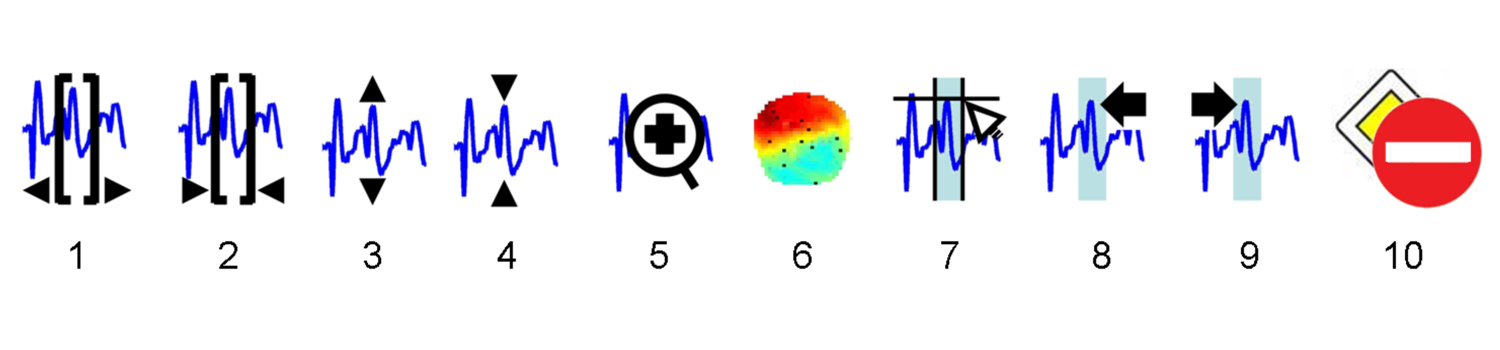
\includegraphics[width=100mm]{meeg/jeandisplay}
\end{center}
\caption{\em SPM EEG REVIEW buttons legend 1-2: increase/decrease width of plotted time window, 3-4: increase/decrease global scaling display factor, 5: zoom in, 7: add event, 8-9: scroll backward/forward data from marker to marker, 10: declare event as good/bad} 
\end{figure}

\section{Batching and scripts}
Although all functions can be called by the GUI, the sole use 
of the GUI for preprocessing multi-subject data is a cumbersome 
and error-prone affair. For this reason, we have put in some functions 
into SPM8 which should make batching of otherwise very interactive jobs 
feasible, with no or a minimum amount of matlab knowledge.
How would one batch a series of preprocessing steps in SPM8? 
There are two ways of doing this, the new batch system of SPM8, and generating scripts. 

\subsection{The new SPM8 batch system}
The first uses the new SPM8 batch system described in chapter \ref{Chap:batch_interface}. 
Using this batch system, you can put together a series of processing
steps by choosing options from menus, in any order you like. 
When the full 'job' is specified which may be a sequence of several 
processing step, one executes the job. We will provide a full example
job in the full version of SPM8 (some new functions will be added after the release of SPM8beta). 


\subsection{Script generation}
Another way of batching jobs is by using scripts, written in Matlab. 
In SPM8, you can generate these scripts automatically. 
To do this, you have first to analyze one data set using the 
GUI or the batch system. In SPM8, whenever a preprocessing 
function is called, all the input arguments, once they have been 
assembled by the GUI, are stored in a history. This history 
can then be used to not only see in detail which functions have
been used on a data set, but also to generate a script that 
repeats the same analysis steps. The big difference is that,
this time, no more GUI interactions are necessary because
the script has already all the input arguments which you gave
during the first run. The history of an M/EEG object can be 
accessed by D.history. To generate a script from this history,
execute the command \textit{spm\_eeg\_hist2script;} in Matlab, and 
ou are asked for the file from which you want to extract the history 
and a filename of the new script. Alternatively, 
you can write: \textit{S.history = D.history; S.fname = 'test.m'; spm\_eeg\_hist2script(S);}.
This will generate a script called \textit{test.m}, which, when run, repeats the analysis for the M/EEG object $D$. 
\\
\\
Of course, this script can not only be used to repeat an analysis, 
but the script can also be seen as a template that can be re-used 
for other analyses. One needs minimal matlab knowledge for these changes. 
For example, you can replace the filenames to preprocess a different subject.
Or you can change parameters and then re-run the analysis. We have prepared 
an example, using the same example data set, as in the previous subsection to
demonstrate this (see the file \textit{/man/example\_scripts/histexample.m}). 
Note that these scripts can currently be used to do things that one couldn't 
do with the batch system. For example, if you want to exclude a channel from 
the analysis, there is no way to do this using via the batch system. In the 
GUI, you would have to call display and switch the channel to 'bad'. With a 
script, you simply add a line like \textit{D=badchannels(D, 23, 1)}, which 
flags channel 23 as bad (see also our example script after the filtering step). 
In summary, the idea is to preprocess a file through the GUI or batch system, 
then use the history-function to generate a template, and finally adapt this 
template to modify the analysis in some way. To run the example script on your
computer, you need the data set. Because this is 200 MB in filesize, please
download it from the SPM webpage (http://www.fil.ion.ucl.ac.uk/spm/data/eeg\_mmn/).